\chapter{Metodoloxía e planificación}
\label{chap:metodoloxia_plan}


\lettrine{O}{} obxectivo deste capítulo é explicar como se traballou, as fases e tarefas deste proxecto, como se realizou o seguemento do proxecto e cal sería o custo deste.


\section{Metodoloxía}
\label{sec:metodoloxía}
O método de traballo foi incremental, dividindo as tarefas en partes independentes que foron implementadas, simuladas e verificadas por orde de complexidade antes de proceder coa seguinte.

O procedemento habitual foi dunha reunión semanal na que se revisaba o feito anteriormente, acompañado da comprobación cos tests correspondentes para esa parte. Despois, decidíase cal era o seguinte paso, podendo ser a implementación dunha nova extensión ou modificar un módulo do simulador. Sendo as fases principais estas:

\begin{itemize}
    \item Estudio da documentación existente sobre RISC-V.
    \item Familiarización coa implementación base de RV32I en SystemC. 
    \item Modelado e simulación do multiplicador e divisor de enteiros. 
    \item Modelado e simulación da extensión de punto flotante F. 
    \item Modelado e simulación das extensións Zicsr e  Zifencei.
    \item Empaquetamento do software. 

\end{itemize}

En canto á organización do proxecto, establecéronse unhas tarefas básicas a realizar. Creouse un plan inicial, como foi explicado no anteproxecto. Sen embargo, non se puido cumprir na súa totalidade pola subestimación do tempo necesario para completar ditas actividades. Como consecuencia disto, a implementación das extensións A e D non puido ser realizada. 

En canto ó seguimento do proxecto, creouse un diagrama de Gantt coas actividades a realizar, que se foi actualizando para eliminar as descartadas. 

\begin{figure}[hp!]
  \centering
  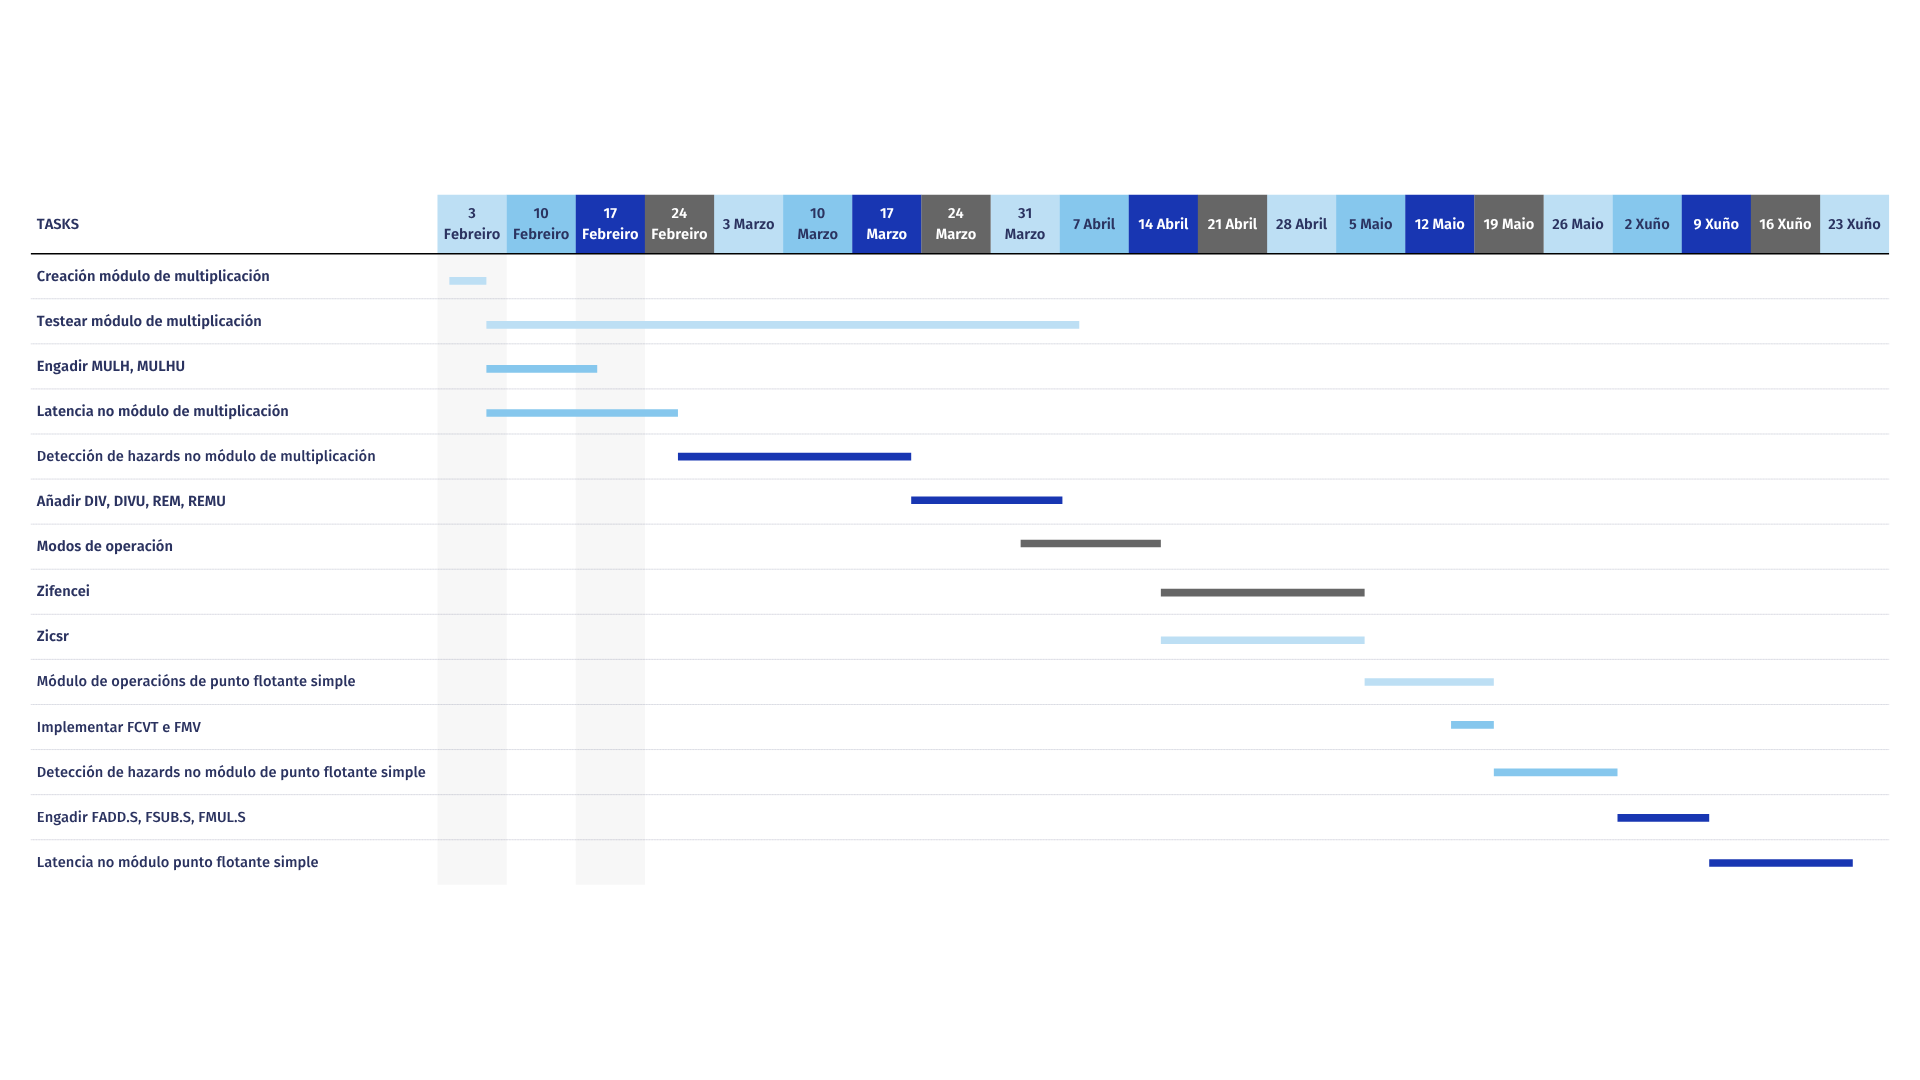
\includegraphics[width=\textwidth]{imaxes/Gantt - TFG.png}
  \caption{Esquema sobre o pipeline do módulo de multiplicación.}
  \label{fig:gantt}
\end{figure}

\section{Presuposto}\label{sec:presuposto}
Para determinar o custo do desenvolvemento do proxecto sería necesario calcular primeiro as horas dedicadas por parte do estudante e do titor e coñecer os prezos destas. Para iso, o BOE ~\cite{boe} establece uns valores mínimos que resultan en 15€/hora para o estudante e 19€/hora para o titor. Na táboa \ref{tab:salario} vése o resultado dos cálculos pertinentes.

\begin{table}[hp!]
    \centering
    \rowcolors{2}{white}{udcgray!25}
    \begin{tabular}{c|c|c|c}
    \rowcolor{udcpink!25}
    \textbf{Persoa} & \textbf{horas}  & \textbf{custo/h} & \textbf{total} 
    \\\hline
    \textit{Estudante} & 240 & 15€/h & 3.600€\\
    \textit{Titor} & 35 & 19€/h & 665€\\
    \multicolumn{3}{c|}{\textbf{Resultado}} & \textit{4.265€} \\
    \end{tabular}
    \caption{Táboa co custo/h e total dos traballadores implicados.}
    \label{tab:salario}
\end{table}

Ademais, é necesario engadir os gastos en licenzas e materiais inventariables. Neste caso, todas as ferramentas empregadas foron gratuítas e non se empregaron recursos adicionais máis aló do portátil, cun valor de 600€. O resultado final móstrase na táboa \ref{tab:precio_final}, sendo de 4.865€.

\begin{table}[hp!]
    \centering
    \rowcolors{2}{white}{udcgray!25}
    \begin{tabular}{c|c}
    \rowcolor{udcpink!25}
    \textbf{Recurso} & \textbf{Prezo} 
    \\\hline
    \textit{Man de obra} & 4.265€\\
    \textit{Materiais e licenzas} & 600€\\
    \textbf{Resultado} & 4.865€ \\
    \end{tabular}
    \caption{Táboa co resultado do custo total do proxecto.}
    \label{tab:precio_final}
\end{table}